\documentclass{article}
\usepackage{amsthm}
\usepackage{graphicx}
\usepackage{ctex}
\usepackage{amsmath}
\usepackage{amssymb} % 添加 amssymb 以支持更多符号
\usepackage{amsfonts}
\usepackage{tikz}
\usepackage{cancel}
\usepackage{listings}
\usetikzlibrary{arrows.meta} % 箭头样式
\title{离散数学作业\_4.2}
\author{李云浩 241880324}
\date{\today}
\lstset{
    language=C++, % 设置语言
    basicstyle=\ttfamily\small, % 基本字体
    numbers=left, % 行号在左侧
    numberstyle=\tiny\color{gray}, % 行号样式
    frame=single, % 边框
    captionpos=b, % 标题位置(底部)
    breaklines=true, % 自动换行
    keywordstyle=\color{blue}, % 关键字颜色
    commentstyle=\color{ForestGreen}, % 注释颜色
    stringstyle=\color{red}, % 字符串颜色
    tabsize=4 % 制表符替换为4空格
}
\begin{document}
\maketitle
\section{4.6}
\subsection{T2}
\begin{lstlisting}
    EDGE(i ,j){
        int ptr = VERT[i];
        while(NEXT[ptr] != 0){
            if(HEAD[ptr] == j){
                return T;
            }
            ptr = NEXT[ptr];
        }
        if(NEXT[ptr] == 0 && HEAD[ptr] == j) return T;
        else return F;
    }
\end{lstlisting}
\subsection{T3}
因为$R$一共有$P$条边,$N$个顶点。因此平均每个顶点的出度为$\frac{P}{N}$。对这$\frac{P}{N}$个出度进行排序,
如果要找的边为第$n$条,则需要$n$步,如果找的边不存在,那么则需要$\frac{P}{N}$步。
因此平均步数为:$\frac{1 + 2 + \dots + \frac{P}{N} + (N - \frac{P}{N})(\frac{P}{N})}{N} = \frac{(2N - \frac{P}{N} + 1)(\frac{P}{N})}{2N}$
\subsection{T4}
\begin{lstlisting}
    LOOK(NUM, NEXT, START, N, K){
        int ptr = START;
        while(NEXT[ptr] != 0){
            if(NUM[ptr] == K) return ptr;
            else ptr == NEXT[ptr];
        }
        if(NUM[ptr] != K) print("NOT FOUND");
        else return ptr;
    }
\end{lstlisting}
\subsection{T6}
$$
\begin{array}{|c|c|c|c|}
    VERT & TAIL & HEAD & NEXT\\
    \hline
    2 & 4 & 1 & 9\\
    4 & 1 & 1 & 3 \\
    7 & 1 & 2 & 5\\
    1 & 2 & 1 & 6\\
    \  & 1 & 3 & 0\\
    \  & 2 & 4 & 8\\
    \  & 3 & 4 & 10\\
    \  & 2 & 3 & 0\\
    \  & 4 & 3 & 0\\
    \  & 3 & 3 & 0
\end{array}
$$
\subsection{T8}
1.有向图:\\
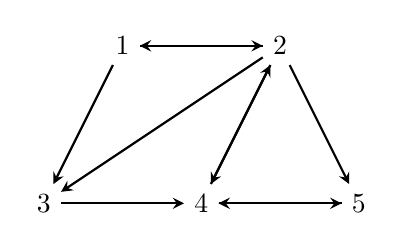
\begin{tikzpicture}[->, thick, >=stealth, node distance=2.5cm]
    \node (1) at (2,2) {1};
    \node (2) at (4,2) {2};
    \node (3) at (1,0) {3};
    \node (4) at (3,0) {4};
    \node (5) at (5,0) {5};

    \draw (1) -- (2);
    \draw (1) -- (3);
    \draw (2) -- (1);
    \draw (2) -- (3);
    \draw (2) -- (4);
    \draw (2) -- (5);
    \draw (3) -- (4);
    \draw (4) -- (2);
    \draw (4) -- (5);
    \draw (5) -- (4);
\end{tikzpicture}

2.矩阵:
$$
\begin{bmatrix}
    0 & 1 & 1 & 0 & 0\\
    1 & 0 & 1 & 1 & 1\\
    0 & 0 & 0 & 1 & 0\\
    0 & 1 & 0 & 0 & 1\\
    0 & 0 & 0 & 1 & 0
\end{bmatrix}
$$
\subsection{T12}
$$VERT = [1, 4, 7, 11]$$
$$TAIL = [1, 1, 1, 2, 2, 2, 3, 3, 3, 3, 4, 4, 4]$$
$$HEAD = [1, 2, 4, 1, 2, 4, 1, 2, 3, 4, 1, 2, 4]$$
$$NEXT = [2, 3, 0, 5, 6, 0, 8, 9, 10, 0, 12, 13, 0]$$
\section{4.7}
\subsection{T7}
(a) $\overline{R} = \{(1, 4), (2, 1), (3, 1), (3, 2), (3, 3), (4, 2), (4, 3), (4, 4)\}$\\
(b) $R \cap S = \{(1, 1), (1, 2), (2, 2), (2, 3), (2, 4), (3, 4), (4, 1)\}$\\
(c) $R \cup S = \{(1, 1), (1, 2), (1, 3), (1, 4), (2, 2), (2, 3), (2, 4), (3, 1), (3, 2), (3, 4), (4, 1), (4, 4)\}$\\
(d) $S^{-1} = \{(1, 1), (1, 3), (1, 4), (2, 1), (2, 2), (2, 3), (3, 2), (4, 1), (4, 2), (4, 3), (4, 4)\}$  
\subsection{T8}
(a) $\overline{R} = \{(a, c), (a, e), (b, a), (b, c), (b, d), (c, a), (c, c), (c, d), (c, e), (d, a), (d, b),\\
(d, e), (e, c), (e, d), (e, e)\}$\\
(b) $R \cap S = \{(a, a), (a, d), (c, b), (e, a), (e, b)\}$\\
(c) $R \cup S = \{(a, a), (a, b), (a, d), (a, e), (b, a), (b, b), (b, e), (c, b), (c, d), (d, c), (d, d),\\
(e, a), (e, b), (e, d), (e, e)\}$\\
(d) $S^{-1} = \{(a, a), (a, b), (a, e), (b, c), (b, e), (d, a), (d, c), (d, e), (e, a), (e, e)\}$
\subsection{T12}
(a) $M_{R\cap S} = 
\begin{bmatrix}
    0 & 0 & 0\\
    0 & 0 & 1\\
    0 & 0 & 0\\
    0 & 1 & 0
\end{bmatrix}$\quad
(b) $M_{R \cup S} = 
\begin{bmatrix}
    1 & 1 & 1\\
    1 & 1 & 1\\
    0 & 1 & 1\\
    1 & 1 & 1
\end{bmatrix}$\\
(c) $R^{-1} = 
\begin{bmatrix}
    0 & 0 & 0 & 1\\
    1 & 1 & 0 & 1\\
    0 & 1 & 1 & 1
\end{bmatrix}$\quad
(d) $M_{\overline{S}} = 
\begin{bmatrix}
    0 & 1 & 0\\
    0 & 1 & 0\\
    1 & 0 & 1\\
    1 & 0 & 1
\end{bmatrix}$
\subsection{T14}
$R\cap S = \{(1, 1), (1, 2), (2, 1), (2, 2), (3, 3), (4, 4), (5, 5), (6, 6)\}$\\
划分:$\{\{1, 2\}, \{3\}, \{4\}, \{5\}, \{6\}\}$。
\subsection{T19}
因为闭包运算是往集合里面添加元素的过程,相当于让关系矩阵中的部分的0变为1,但是不能把1变为0。
因此例如一个等价关系,往里面不断将0化为1,都不能使其具有非自反、非对称、反对称关系。
因此闭包的概念不适用于非自反、非对称、反对称之中。
\subsection{T20}
(a) $R \circ S = \{(a, c) | a \leq 6c\}$。因为$2 \leq 6 \times 3 = 18$,因此$(2, 3) \in R \circ S$。\\
(b) 因为$8 \geq 6 \times 1$,因此$(8, 1) \notin R \circ S$
\subsection{T23}
(a) 自反性:假设$R$, $S$是$A$上的关系,且都具有自反性。$\forall x \in A \rightarrow (x, x) \in R \land (x, x) \in S$.
所以对于$R \circ S$而言,有$\forall x \in A, (x, x) \circ (x, x) = (x, x)$。因此$R \circ S$仍为自反的。\\
反自反性:假设$R = \{(1, 2)\}, S = \{(2, 1)\}$,则$R \circ S = \{(1, 1)\}$。反自反不能保持
对称性:假设$R = \{(1, 2), (2, 1)\}, S = \{(2, 3), (3, 2)\}$,则$R \circ S = \{(1, 3)\}$,对称性不能保持。\\
反对称性:假设$R = \{(1, 2), (2, 2)\}, S = \{(2, 2), (1, 1), (2, 1)\}$,则$R \circ S = \{(1, 2), (1, 1), (2, 2), (2, 1)\}$,
反对称性不能保留
传递性:假设$R = \{(1, 2), (2, 4)\}, S = \{(2, 2), (4, 3)\}$,则$R \circ S = \{(1, 2), (2, 3)\}$,对称性不能保持。\\
(b) 自反性:根据(a)中可知,自反性质能够保留,因此$S \circ R$是$A$上的自反关系。\\
对称性:假设$R = \{(1, 1), (1, 2), (2, 1), (2, 2), (3, 3)\}, S = \{(1, 1), (2, 2), (2, 3), (3, 2), (3, 3)\}$。
所以$S \circ R = \{(1, 1), (1, 2), (1, 3), (2, 1), (2, 2), (2, 3), (3, 3), (3, 2)\}$,不满足对称性。
因此$S \circ R$不是A上的等价关系
\subsection{T24}
(a) $M_{R \circ R}= 
\begin{bmatrix}
    1 & 1 & 1 & 1 & 1\\
    1 & 1 & 1 & 1 & 0\\
    1 & 0 & 1 & 1 & 1\\
    1 & 0 & 1 & 1 & 1\\
    1 & 1 & 1 & 1 & 1
\end{bmatrix}$ \quad
(b) $M_{S \circ R} = 
\begin{bmatrix}
    1 & 1 & 1 & 1 & 1\\
    1 & 0 & 1 & 0 & 0\\
    1 & 1 & 1 & 1 & 1\\
    1 & 0 & 1 & 1 & 0\\
    1 & 1 & 1 & 1 & 1
\end{bmatrix}$\\
(c) $M_{R \circ S} = 
\begin{bmatrix}
    1 & 0 & 1 & 1 & 1\\
    1 & 0 & 1 & 1 & 1\\
    1 & 0 & 1 & 1 & 1\\
    1 & 1 & 1 & 1 & 1\\
    1 & 1 & 1 & 1 & 1
\end{bmatrix}$ \quad
(d) $M_{S \circ S} = 
\begin{bmatrix}
    1 & 1 & 1 & 1 & 1\\
    1 & 0 & 1 & 1 & 0\\
    1 & 0 & 1 & 1 & 0\\
    1 & 1 & 1 & 1 & 1\\
    1 & 0 & 0 & 1 & 1
\end{bmatrix}$
\subsection{T26}
因为$R \cap R^{-1} = S \cap S^{-1} = \varnothing$,所以
\begin{align*}
    (R \cap S) \cap (R \cap S)^{-1} &= (R \cap S) \cap (R^{-1} \cap S^{-1})\\
    &= (R \cap R^{-1}) \cap (S \cap S^{-1})\\
    &= \varnothing
\end{align*}
因此$R \cap S$是非对称的。
\begin{align*}
    (R \cup S) \cap (R \cup S)^{-1} &= (R \cup S) \cap (R^{-1} \cup S^{-1})\\
    &= ((R \cup S) \cap R^{-1}) \cup ((R \cup S) \cap S^{-1})\\
    &= R \cap R^{-1} \cup S \cap R^{-1} \cup R \cap S^{-1} \cup S \cap S^{-1}\\
    &= S \cap R^{-1} \cup R \cap S^{-1}\\
    &= S \cap R^{-1} \cup (S \cap R^{-1})^{-1}
\end{align*}
因此,如果$S \cap R^{- 1} = \varnothing$,$R \cup S$是非对称的,反之则不是。
\subsection{T27}
假设$R = \{(1, 1), (1, 2), (2, 2)\}, S = \{(1, 1), (2, 2), (2, 1)\}$。因此
$R \cup S = \{(1, 1), (1, 2), (2, 1), (2, 2)\}$是对称的,不是反对称的。\\
对于$R \cap S$,如果$\forall (a, b) ((a, b) \in  (R \cap S) \land (b, a) \in (R \cap S))$,故$(a, b) \in R \land (b, a) \in R$。
因为$R$是反对称的,因此$a = b$,故$R \cap S$是反对称的。
\subsection{T28}
对$\forall a \in A, c \in C$,有$a (S \cup T) \circ R c$
\begin{align*}
    a(S \cup T) \circ Rc &\Leftrightarrow (\exists b \in B)(a(S \cup T)b \land bRc)\\
    &\Leftrightarrow (\exists b \in B)((aSb \lor aTb) \land bRc)\\
    &\Leftrightarrow (\exists b \in B)(aSb \land bRc \lor aTb \land bRc)\\
    &\Leftrightarrow (\exists b \in B)(a S \circ R c \lor a T \circ R c)\\
    &\Leftrightarrow (a (S \circ R) \cup (T \circ R)c)
\end{align*}因此$(S \cup T)\circ R = (S \circ R) \cup (T \circ R)$
\subsection{T30}
$\forall a \in A, c \in C$,有$a T \circ R c$.
\begin{align*}
    a T \circ R c &\Rightarrow (\exists b \in B)(aTb \land bRc)\\
    &\Rightarrow (\exists b \in B)(aTb \land bSc)\\
    &\Rightarrow a T \circ S b
\end{align*}因此:$T \circ R \subseteq T \circ S$
\subsection{T31}
(a) 因为$\forall a \in A, b \in A, a(R \cap S)b \Leftrightarrow aRb \land aSb$。
因此$(a, b) \in (R \cap S) \Leftrightarrow (a, b) \in R \land (a, b) \in S$,
故$M_{R\cap S} = M_R \land M_S$\\
(b) 因为$\forall a \in A, b \in A, a(R \cup S)b \Leftrightarrow aRb \lor aSb$。
因此$(a, b) \in (R \cup S) \Leftrightarrow (a, b) \in R \lor (a, b) \in S$,
故$M_{R \cup S} = M_R \lor M_S$\\
(c) 因为$\forall a \in A, b \in A, (a, b) \in R^{-1} \Leftrightarrow (b, a) \in R$,
故$M_{R^{-1}} = (M_R)^T$\\
(d) 因为$\forall a \in A, b \in A, (a, b) \in \overline{R} \Leftrightarrow (a, b) \notin R$,
故$M_{\overline{R}} = \overline{M_R}$
\subsection{T36}
$\forall (a, b) \in R \land (a, b) \notin S$因为$R,S$都是对称的,因此$(b, a) \in R \land (b, a) \notin S$。
故$\forall (a, b) \in R \land (a, b) \notin S \Rightarrow (b, a) \in R \land (b, a) \notin S$。
因此$\forall (a, b) \in (R - S) \Rightarrow (b, a) \in (R - S)$,即$R - S$也是一个对称关系。
\subsection{T37}
(a) 充分性:$R$是对称的 $\Rightarrow R = R^{-1}$\\
$\forall (b, a) \in R \Rightarrow (a, b) \in R^{-1}$,又因为$R$是对称的,
因此$\forall (b, a) \in R \Rightarrow (a, b) \in R$。因此$R \subseteq R^{-1}$。
同理$R^{-1} \subseteq R$,因此$R = R^{-1}$。\\
必要性:$R = R^{-1} \Rightarrow R$ 是对称的\\
因为$R = R^{-1}$,$\forall (a, b) \in R \Rightarrow (a, b) \in R^{-1}$,又因为
$\forall (a, b) \in R^{-1} \Rightarrow (b, a) \in R$。因此$\forall (a, b) \in R \Rightarrow (b, a) \in R$。
故$R$是对称的。

(b) 充分性:$R$是反对称的 $\Rightarrow R \cap R^{-1} \subseteq \Delta$\\
$\forall a \in A, b \in B$,\\
当$a \neq b$时,$\forall (a, b) \in R \Rightarrow (b, a) \notin R \Rightarrow (a, b) \notin R^{-1}$。
因此$R \cap R^{-1} = \varnothing$。\\
当$a = b$时,$\forall (a, b) \in R \Rightarrow (b, a) \in R \Rightarrow (a, b) \in R^{-1}$,
因此$R \cap R^{-1} \subseteq \Delta$。\\
综上所述:$R$是反对称的 $\Rightarrow R \cap R^{-1} \subseteq \Delta$\\
必要性:$R \cap R^{-1} \subseteq \Delta \Rightarrow R$ 是反对称的\\
$\forall a \in A, b \in B$,\\
当$a \neq b$时,$\forall (a, b) \in R \Rightarrow (a, b) \notin R^{-1} \Rightarrow (b, a) \notin R$。
因此$\forall a \in A, \nexists b(b \in A \land b \neq a) \Rightarrow (a, b) \in R \land (b, a) \in R$\\
当$a = b$时,$\forall (a, b) \in R \Rightarrow (b, a) \in R \Rightarrow (a, b) \in R^{-1}$。\\
综上所述:$R \cap R^{-1} \subseteq \Delta \Rightarrow R$ 是反对称的\\
(c) 充分性:$R$是非对称的 $\Rightarrow R \cap R^{-1} = \varnothing$\\
因为$R$是非对称的,因此$\forall (a, b) \in R \Rightarrow (b, a) \notin R \Rightarrow (a, b) \notin R^{-1}$,
故$R \cap R^{-1} = \varnothing$\\
必要性:$R \cap R^{-1} = \varnothing \Rightarrow R$ 是非对称的\\
因为$R \cap R^{-1} = \varnothing$,因此$\forall (a, b) \in R \Rightarrow (a, b) \notin R^{-1} \Rightarrow (b, a) \notin R$,
因此$R$是非对称的。\\
\section{4.8}
\subsection{T8}
充分性:$a S^{\infty} b \Rightarrow R$中存在从$a$到$b$的一条路径,且该路径具有偶数条边。\\
因为$S = R^2$,因为$a S^{\infty}b \Rightarrow \exists i \geq 1 s.t. a S^i b$。
又因为$S^i = R^{2i}$,所以存在一条从$a$到$b$长度为$2i$的路径。即$a S^{\infty} b \Rightarrow R$中存在从$a$到$b$的一条路径,且该路径具有偶数条边。\\
必要性:$R$中存在从$a$到$b$的一条路径,且该路径具有偶数条边 $\Rightarrow a S^{\infty} b $\\
因为$R$中存在从$a$到$b$的一条路径,且该路径具有偶数条边。不妨设$aR^{2k}b$,因为$S = R^2$,
故$a S^k b$. 又因为$S^k \subseteq S^{\infty}$,即$a S^{\infty} b$。\\
综上所述:$a S^{\infty} b $当且仅当$ R$中存在从$a$到$b$的一条路径,且该路径具有偶数条边。
\subsection{T10}
$M_R = 
\begin{bmatrix}
    1 & 1 & 0 & 0\\
    1 & 0 & 0 & 0\\
    0 & 0 & 0 & 0\\
    0 & 0 & 1 & 0
\end{bmatrix},\quad 
M_{R^2} = 
\begin{bmatrix}
    1 & 1 & 0 & 0\\
    1 & 0 & 0 & 0\\
    0 & 0 & 0 & 0\\
    0 & 0 & 1 & 0
\end{bmatrix} = M_R$.\\
因此$M_{t(R)} = 
\begin{bmatrix}
    1 & 1 & 0 & 0\\
    1 & 0 & 0 & 0\\
    0 & 0 & 0 & 0\\
    0 & 0 & 1 & 0
\end{bmatrix}$
\subsection{T12}
$M_R = 
\begin{bmatrix}
    0 & 0 & 0 & 1\\
    1 & 0 & 0 & 1\\
    0 & 1 & 0 & 1\\
    0 & 0 & 1 & 0
\end{bmatrix}, \quad
M_{R^2} = 
\begin{bmatrix}
    0 & 0 & 0 & 1\\
    1 & 0 & 0 & 1\\
    1 & 1 & 0 & 1\\
    0 & 0 & 1 & 0
\end{bmatrix}, \quad
M_{R^3} = 
\begin{bmatrix}
    0 & 0 & 0 & 1\\
    1 & 0 & 0 & 1\\
    1 & 1 & 0 & 1\\
    1 & 1 & 1 & 1
\end{bmatrix},$\\
$M_{R^4} = 
\begin{bmatrix}
    1 & 0 & 1 & 1\\
    1 & 0 & 1 & 1\\
    1 & 1 & 1 & 1\\
    0 & 1 & 1 & 1
\end{bmatrix}$
因此:
$M_{t(R)} = 
\begin{bmatrix}
    1 & 0 & 1 & 1\\
    1 & 0 & 1 & 1\\
    1 & 1 & 1 & 1\\
    0 & 1 & 1 & 1
\end{bmatrix}$
\subsection{T14}
$M_R = 
\begin{bmatrix}
    0 & 0 & 0 & 0\\
    1 & 1 & 1 & 0\\
    0 & 1 & 1 & 0\\
    0 & 1 & 0 & 0
\end{bmatrix}$\\
求$M_s{(R)}$的传递闭包关系矩阵:
$M_{s(R)} = 
\begin{bmatrix}
    0 & 1 & 0 & 0\\
    1 & 1 & 1 & 1\\
    0 & 1 & 1 & 0\\
    0 & 1 & 0 & 0
\end{bmatrix}$,
$M_{s(R)^2} = 
\begin{bmatrix}
    1 & 1 & 1 & 1\\
    1 & 1 & 1 & 1\\
    1 & 1 & 1 & 1\\
    1 & 1 & 1 & 1
\end{bmatrix}$
故:$M_{t(s(R))} = 
\begin{bmatrix}
    1 & 1 & 1 & 1\\
    1 & 1 & 1 & 1\\
    1 & 1 & 1 & 1\\
    1 & 1 & 1 & 1
\end{bmatrix}$\\
求$M_{t(R)}$的对称闭包关系矩阵:
$M_{R^2} = 
\begin{bmatrix}
    0 & 0 & 0 & 0\\
    1 & 1 & 1 & 0\\
    1 & 1 & 1 & 0\\
    1 & 1 & 1 & 0
\end{bmatrix}, \quad$
$M_{R^3} = M_{R^2}$.
因此$M_{s(t(R))} = 
\begin{bmatrix}
    0 & 1 & 1 & 1\\
    1 & 1 & 1 & 1\\
    1 & 1 & 1 & 1\\
    1 & 1 & 1 & 0
\end{bmatrix}$
因此:$R_t$的对称闭包和$R_s$的传递闭包不具有相同的关系
\subsection{T18}
$A / R = \{\{1\}, \{2, 3\}, \{4 ,5\}\}, A / S = \{\{1, 2\}, \{3\}, \{4, 5\}\}$.\\
$A / (R \cup S)^\infty = \{\{1, 2, 3\}, \{4, 5\}\}$
\subsection{T20}
因为19题的前提条件是两个关系本身是等价关系,不具有普遍性。而Warshall算法不需要这个前提条件。
\subsection{T23}
使用了直接证明法。先假设$\forall S, (R \subseteq S)$,后续利用$S$的传递性,说明$S^{\infty} \subseteq S$,
又因为满足公式$S^{\infty} = \bigcup_{n = 1}^{\infty}S^n \subseteq S$,结合$R \subseteq S$,推出$R^{\infty} \subseteq
S^{\infty} \subseteq S$。从而证明是传递关系中最小的。
\subsection{T24}
使用了构造性证明法。考虑了路径中可能成环,把成环的部分删去,留下顶点各异的部分。因为顶点数不可能超过n,
因此路径的长度也至多是n。由此证明计算$R^{\infty}$并不需要计算比$n$次幂大的$R$的幂。
\subsection{T25}
设包含$R$的最小等价关系为$S$.\\
$S$满足自反性:$\forall x \in A, (x, x) \in S$。\\
$S$满足对称性且$R \subseteq s$:$\forall a \in A, b \in A \land |a| \leq |b| \Rightarrow (a, b) \in R \Rightarrow (a, b) \in S$,
因为$S$满足对称性,所以$|a| \geq |b| \Rightarrow (a, b)\in S \Rightarrow a \in A, b \in A a \neq b \Rightarrow (a, b) \in S$。\\
综上所述,$\forall a \in A, b \in A.$当$a = b, (a, b) \in S$。当$a \neq b, (a, b) \in S$。
因此,$\forall a \in A, b \in A \Rightarrow (a, b) \in S$即$S = A \times A = \mathbf{R} \times \mathbf{R}$。 

\end{document}